\part[Anhang und Verzeichnise]{Anhänge und Verzeichnise
                  \begin{center}
                     \begin{minipage}[c]{10.7cm}
                        \small Hitobito: Neue Generation von Personen-Filtern \\
                        Autor: Marc Egli
                     \end{minipage}
                  \end{center}
                 }

\chapter{Verzeichnise}

\section{Code}


\listoftables

\listoffigures

\renewcommand\bibname{Quellenverzeichnis}
\begin{thebibliography}{9}
    \bibitem[Github Docs - Understanding connections between repositories]{Github Docs} \url{https://docs.github.com/en/repositories/viewing-activity-and-data-for-your-repository/understanding-connections-between-repositories}, (04.03.2025)
    \bibitem[Github Docs - Configuring issue templates]{Github Docs} \url{https://docs.github.com/en/communities/using-templates-to-encourage-useful-issues-and-pull-requests/configuring-issue-templates-for-your-repository}, (04.03.2025)
    \bibitem[Leo - Translating]{Leo} \url{https://dict.leo.org/german-english}, (04.03.2025)
\end{thebibliography}
\addcontentsline{toc}{subsection}{Quellenverzeichnis}

\chapter{Verwendete Abkürzungen}

\begin{table}[H]
    \rowcolors{2}{puzzleblue!30}{white}
    \begin{tabular}{|L{0.3\textwidth}|L{0.6\textwidth}|}
        \hline
        \rowcolor{puzzleblue} \textbf{\color{white}Abkürzung} & \textbf{\color{white}Bedeutung} \\[12pt]
        \hline
        UML & Unified Modeling Language \\
        \hline
    \end{tabular}
    \caption{Verwendete Abkürzungen}
\end{table}

\chapter{Glossar}

\begin{table}[H]
    \rowcolors{2}{puzzleblue!30}{white}
    \begin{tabular}{|L{0.3\textwidth}|L{0.6\textwidth}|}
        \hline
        \rowcolor{puzzleblue} \textbf{\color{white}Bezeichnung} & \textbf{\color{white}Bedeutung} \\[12pt]
        \hline
        Hitobito & Community Management Tool \\
        \hline
    \end{tabular}
    \caption{Glossar}
\end{table}

\chapter{Anhänge}

\section{Git Commit Message Convention}
\label{sec:gitconv}
\begin{figure}[h]
    \centering
    \fbox{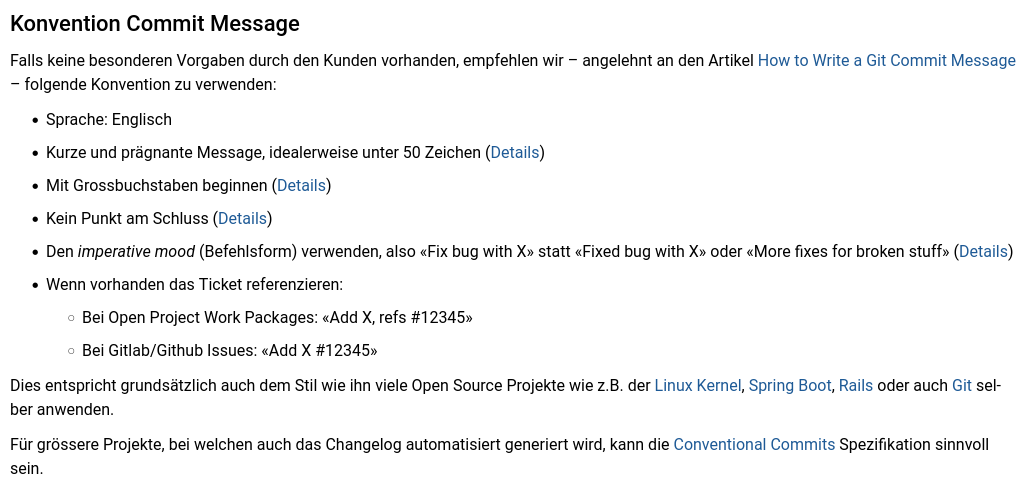
\includegraphics[width=1\textwidth,]{git_commit_conventions.png}}
    \caption{Puzzle ITC Git commit conventions}
\end{figure}

\section{Sitzungsprotokolle}
\section{Git commit convention}
\section{Security conventions}





